% HEAD BEGIN
\documentclass[letterpaper, 12pt]{article}
\usepackage{graphicx}
\usepackage{multicol}
\usepackage{anysize}
\usepackage{fontspec}
\usepackage[fontset=none]{ctex}
\usepackage{tabularx}
\PassOptionsToPackage{hyphens}{url}
\usepackage[breaklinks=true, colorlinks=true]{hyperref}
\expandafter\def\expandafter\UrlBreaks\expandafter{\UrlBreaks\do\a\do\b\do\c\do\d\do\e\do\f\do\g\do\h\do\i\do\j\do\k\do\l\do\m\do\n\do\o\do\p\do\q\do\r\do\s\do\t\do\u\do\v\do\w\do\x\do\y\do\z\do\A\do\B\do\C\do\D\do\E\do\F\do\G\do\H\do\I\do\J\do\K\do\L\do\M\do\N\do\O\do\P\do\Q\do\R\do\S\do\T\do\U\do\V\do\W\do\X\do\Y\do\Z}
% \let\oldurl\url
% \renewcommand{\url}[1]{\begin{sloppypar}\oldurl{#1}\end{sloppypar}}
\setlength\columnsep{30pt}
\marginsize{30pt}{30pt}{10pt}{20pt}
\setmainfont{TeX Gyre Bonum}
\setCJKmainfont[BoldFont=Noto Serif CJK SC Bold, ItalicFont=FandolKai]{Noto Sans CJK SC}
\setlength{\parindent}{0cm}
% \setCJKmonofont{Noto Sans CJK SC}
\begin{document}
\begin{center}
    \Huge\textbf{南哪大专醒前消息}
\end{center}
\vspace{4mm}
\hrule
\renewcommand\tabularxcolumn[1]{m{#1}}
\begin{tabularx}{\textwidth}{>{\hsize.2\hsize}X>{\hsize.6\hsize}X>{\hsize.2\hsize}X}
    \begin{flushleft}
        2024.9.30\, No.75
    \end{flushleft}
    &
    \begin{center}
        \textit{“克明峻德。”}
    \end{center}
    &
    \begin{flushright}
        \textbf{南京市栖霞区}
    \end{flushright}
\end{tabularx}
\vspace{-3.5mm}
\hrule
\vspace{4mm}
% HEAD END
\centerline{\huge\textbf{活动预告}}
\begin{multicols}{2}

\section{Deadline Ongoing}
\begin{tabular}{|c|c|c|}
    \hline
    消息(未见ddl的,不刊) & 截止日期 & 刊载日期\\
    \hline\hline
    仙林校史馆招募讲解员 & 10.30 & 9.12\\
    国优计划报名 & 10.7 & 9.19\\
    本科生暑期课程评教 & 10.31 & 9.19\\
    网易雷火大赛 & 10.7 & 9.22\\
    大创训练计划申报 & 11.18 & 9.24\\
    苏州校区音乐会 & 10.19 & 9.25\\
    外院国庆摄影征集 & 10.7 & 9.25\\
    多阅志愿者招募 & 10.1 & 9.26\\
    雨花成长计划课堂报名 & 10.3 & 9.26\\
    港澳台生中华文化大赛 & 10.9 & 9.26\\
    心理中心征稿 & 10.10 & 9.28\\
    周末剧场 & 10.10 & 9.28\\
    历史学院国庆活动 & 10.7 & 9.28\\
    计院国庆桌游会 & 10.5 & 9.29\\
    台湾地区交换项目 & 10.7 & 9.29\\
    图书馆小放送 & 10.1 & 9.29\\
    第十九届大挑 & 10.15 & 9.30\\
    声谷创新基金 & 10.18 & 9.30\\
    软院国庆桌游会 & 10.7 & 9.30\\
    物院观影会 & 10.3 & 9.30\\
    国际化处全媒体招新 & 10.8 & 9.30\\
    午餐读书会 & 10.10 & 9.30\\
    “周一剧!”第二期 & 10.5 & 9.30\\
    \hline
\end{tabular}
\section{编辑部招聘人才}
编辑部招聘人才,用爱发电,工作轻松,详情可联系QQ:1329527951 客服小祥\\想订阅本消息或获取PDF版(便于查看超链接),可加QQ群:\href{https://qm.qq.com/q/FGX1VYCrGS}{962626571}.
\section{讲座}
\begin{tabular}{|c|c|c|}
    \hline
    往期讲座 & 开展日期 & 刊载日期\\
    \hline\hline
      \hline
\end{tabular}\\\\


\section{2024大挑}
校团委现通知“proposal大挑战”暨第十九届“挑战杯”全国大学生课外学术科技作品竞赛主体赛项目征集事宜。\\

各学院组织团队学生填写申报材料上交所在学院团委,跨学院项目由项目第一作者向其所在学院申报。各学院对参赛项目进行审查确认,并于2024年10月15日(星期二)24∶00前提交推荐团队的作品申报书(附件2,Word版和PDF盖章版)、学院推荐汇总表(附件3,Excel版和PDF盖章版),打包发送至校团委学术与“双创”部公共邮箱,邮件标题命名为“学院+‘挑战杯’proposal”。\\
大挑交流群:771567993\\
详见:\url{https://mp.weixin.qq.com/s/z2VWDZQ8WQhrNQEG-SvceQ}

\section{本学期“午餐读书会”情况}
新生学院、高研院、南大出版社现通知午餐读书会事宜。该读书会计划从10月23日开始每周三中午12:20—13:30在南京大学出版社举行,共7讲,以午餐会形式开展。\\
选读书目包括:福柯:《规训与惩罚》。娜塔莉·泽蒙·戴维斯:《马丁·盖尔归来》。《德意志意识形态(节选)》。米歇尔、汉森主编:《媒介研究批评术语集》等。\\
现面向秉文书院和行知书院招募读书会常驻成员,其中秉文书院和行知书院各7名。\\
要求:\\
1. 保证能参加7场读书会。\\
2. 选择其中一本书并在该场读书会进行读书汇报,每次读书会两位汇报人。课后汇报人须撰写所分享书目的读书报告并在两周内上交。常驻成员的读书报告最终将进行院内评优并被编辑成册。\\
3. 具有独立思考的能力、对科研存在一定兴趣.\\
报名表:\url{https://f.wps.cn/g/Q3omKiSK}截止日期为10月10日中午 12:00 。
\section{中国声谷创新基金}
南大双创办启动第二批常熟市“苏州·中国声谷创新基金”成果孵化项目申报工作。通过评审立项的项目将成为江苏省概念验证中心(南京大学)概念验证项目,获得资金扶持、人员培训、项目辅导、孵化和投资等服务。支持方向包括:\\

声学及通信、新能源汽车、先进材料、低空经济、综合产业.

要求较为苛刻,详见:\url{https://mp.weixin.qq.com/s/e0bbtTAWyk1U8B3E0HljKg}。项目申报材料提交截止时间为2024年10月18日(周五),地点为元化路8号南大科学园双创园2栋3楼。
\section{南大全球交流全媒体中心招新}
对象:南京大学全体在读的全日制本科生、硕士生、博士生\\
报名时间:即日起至10月8日\\
具体链接:\url{https://mp.weixin.qq.com/s/IQn0XkzI-B2Y1fYwX_aX_Q}
\section{软院国庆桌游会}
%🤩软!院!也!有!桌!游!会!啦!🤩 \\
%🙈不懂游戏规则怎么办? 🎉没关系,我们配有专人教学!\\
%🙈游戏缺少主持人怎么办? 🎉没关系,我们配有专人主持!\\
%🥳更有我们精心准备的零食饮品等着你💖😍 \\
软院学生会邀请你欢度国庆!\\
专人教学,专人主持,另有零食饮品。\\
时间:【10月7日下午13:00-19:00】\\ 
地点:【费彝民楼B501】\\
感兴趣的同学加群:\\
\url{https://qm.qq.com/q/NdGAqhSZig}

\section{物院国庆活动}
包括“三行情诗赞祖国”,“我和国旗合张影”和“忆峥嵘岁月”电影放映活动。\\
后者将于10月3、4日19:00-21:00在物理楼356播放《志愿军:雄兵出击》,每场不超过60人,会准备零食爆米花。\\
具体情况和报名链接见原文:\url{https://mp.weixin.qq.com/s/LM7q-n1tB5Jbm0yg1b5p6g}

\section{图书馆招募AI达人}
图书馆现发起人工智能相关活动(内含双重福利),向广大师生征集人工智能活动意见与建议,欢迎关注和参与。\\
详情请点击链接\url{https://mp.weixin.qq.com/s/kCYZ-WgoBmHSwbqQ_D8TkA}了解。\\
\section{多个马理论会议、论坛征稿}
近期有多个马克思主义理论学科论坛、会议、期刊等征稿,截止日期分布在本月各旬。因主要面向研究生,故不予详细刊载,可详阅:\url{https://mp.weixin.qq.com/s/hTa7sh2Yee8i_tLwDP5-lA}。

\section{国庆/鼓楼/猫鼠游戏}
南哪表白墙9月30日第12条帖子中,po主提出征集在国庆期间想玩猫鼠游戏的鼓楼校区同学,详情可加群了解,男女不限。qq群聊:\url{https://qm.qq.com/q/i4MKVcJZ60
}
\section{“周一剧!”第二期}
南京大学前社团II剧现通知招募事宜。

小组的规则:

这会是一个持续一个月的学习小组(10.7~10.31)。每周看一个作品,看完之后在群内打卡,分享感受,提出问题。此外因为只有四周,所以有一次不打卡就会被移出微信群。如果有空的话会组织放映会,或者私下约着看。

主题:战后日本。

详见:\url{https://mp.weixin.qq.com/s/FcIIYRr-ECcFtFCU1-zGsQ}问卷截止到10月5日晚23点59分。

\section{“南小宝”秋招}
据“南小宝crush”公众号称,该团队要招募南京大学同学加入。推送全系空文,未见任何详情。原文见:\url{https://mp.weixin.qq.com/s/JBYOb-b6u1TqPzfPHh33gQ}
\end{multicols} 


\hrule
\vspace{4mm}
% APPENDIX BEGIN
\centerline{\huge\textbf{附录}}
\begin{figure}[htbp]
    \centering
    \begin{minipage}[b]{0.32\textwidth}
        \centering
         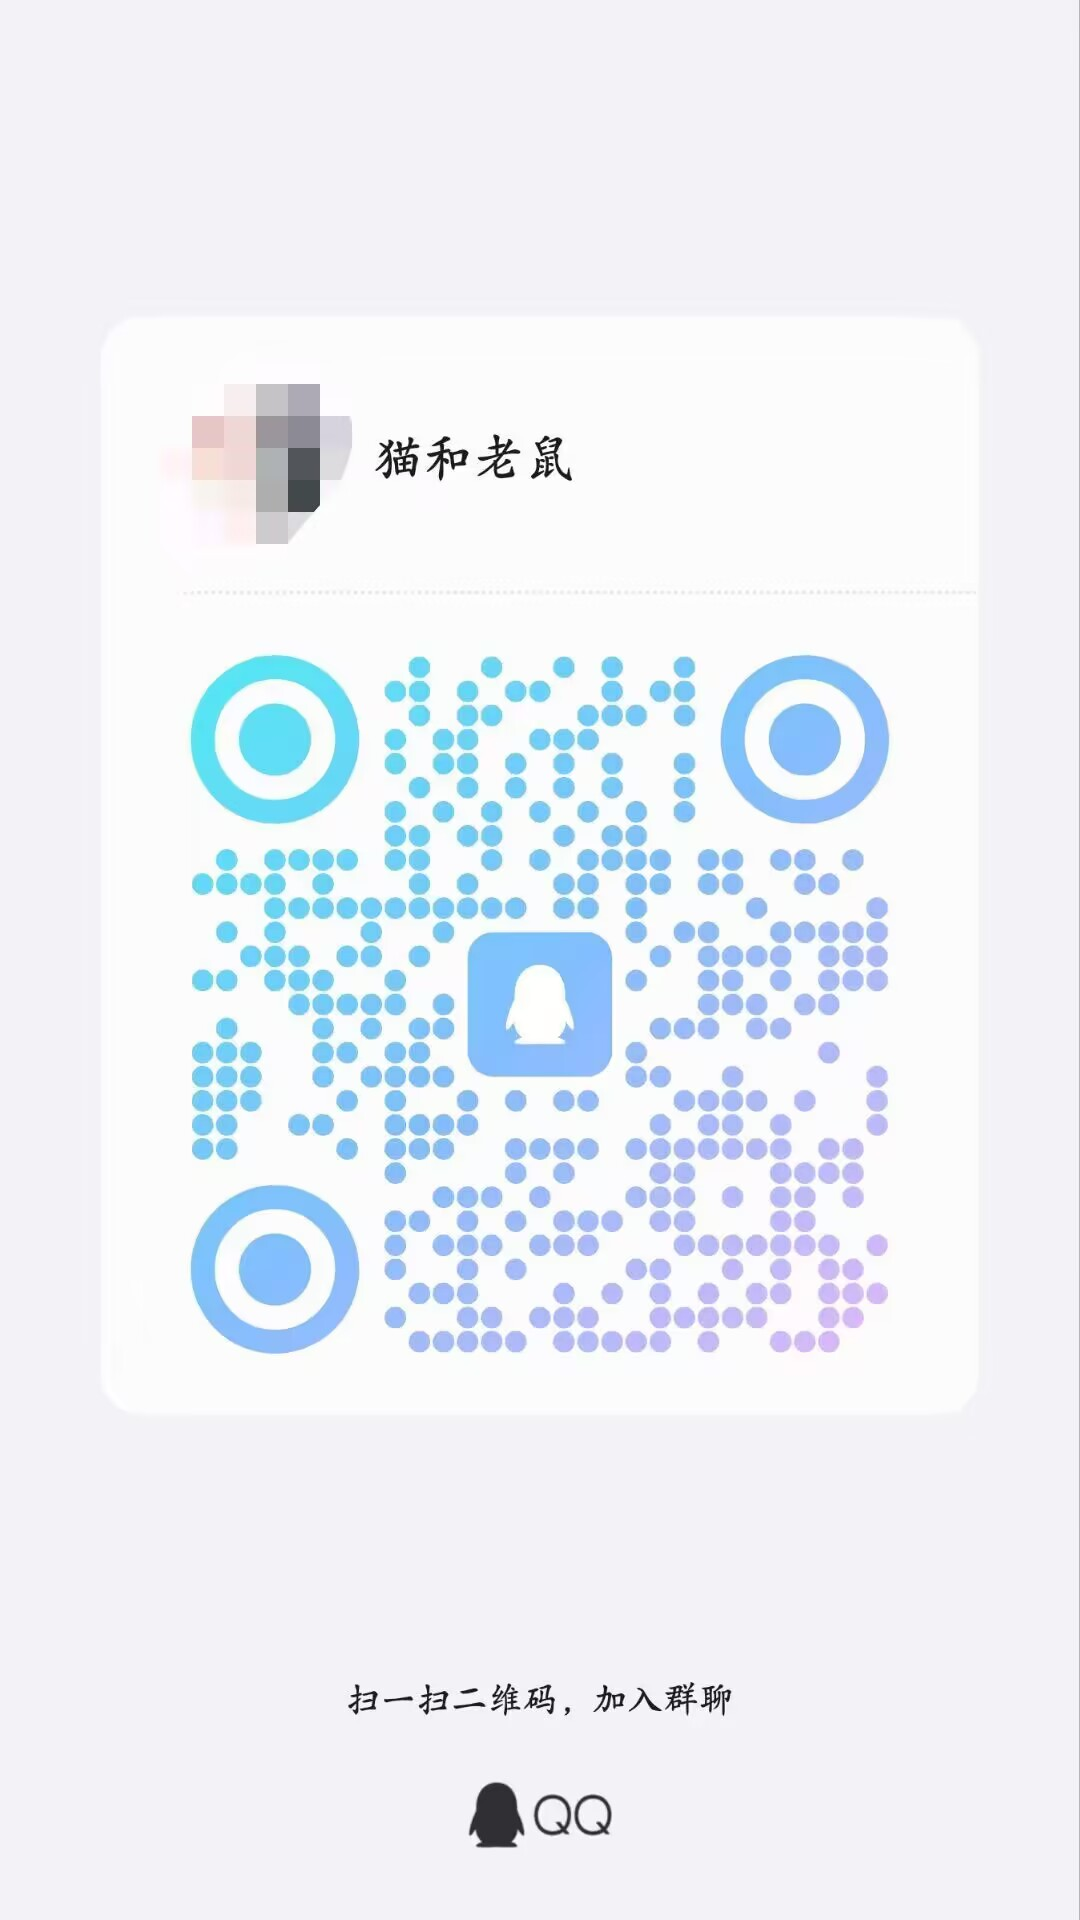
\includegraphics[width=0.5\textwidth]{猫和老鼠.jpg}
        \caption{“猫鼠游戏”}
    \end{minipage}
\end{figure}
\end{document}